\documentclass{standalone}
\usepackage{pgfplots}
\pgfplotsset{compat=newest}
\begin{document}
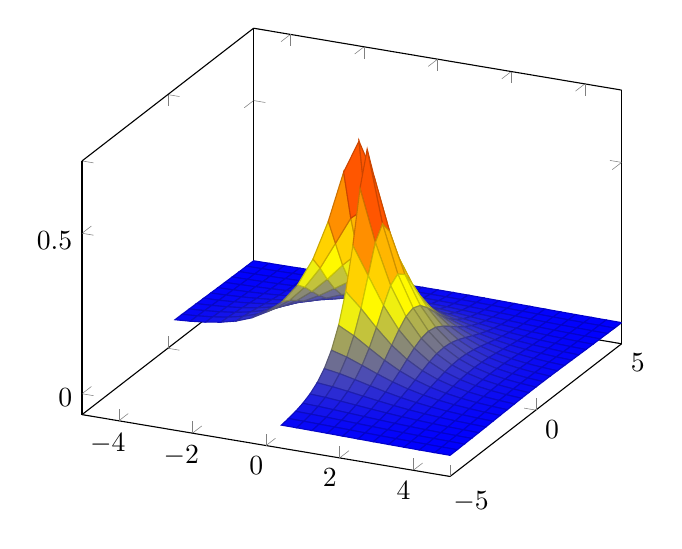
\begin{tikzpicture}
\begin{axis}[
  unbounded coords=jump,
  % A technical filter to cut out 
  % the x<0 and y<0 edge.
  filter point/.code={%
    \pgfmathparse
      {\pgfkeysvalueof{/data point/x}<0}%
    \ifpgfmathfloatcomparison
      \pgfmathparse
        {\pgfkeysvalueof{/data point/y}<0}%
      \ifpgfmathfloatcomparison
        \pgfkeyssetvalue{/data point/x}{nan}%
      \fi
    \fi
  },
  ]
  \addplot3[surf] {exp(-sqrt(x^2 + y^2))};
\end{axis}
\end{tikzpicture}
\end{document}
